%!TEX root = ../thesis.tex
%*******************************************************************************
%****************************** Third Chapter **********************************
%*******************************************************************************
\chapter{Structures in SAT} \label{chap:structure}

% **************************** Define Graphics Path **************************
\ifpdf
    \graphicspath{{Chapter5/Figs/Raster/}{Chapter5/Figs/PDF/}{Chapter5/Figs/}}
\else
    \graphicspath{{Chapter5/Figs/Vector/}{Chapte5/Figs/}}
\fi

\section*{Introduction}
In this chapter we attempt to provide an explanation of why it is simultaneously
possible to have fast ``in practice'' SAT solving algorithms, as seen in Chapter
\ref{chap:solvers}, and also have standing conjectures about the complexity of
SAT that suggest that we should not expect to solve SAT in subexponential time,
as seen in Chapter \ref{chap:complexity}. From this it seems that many SAT instances
are significantly easier than their worst-case counterparts.

This discrepancy between the hardness of the worst-case instances and the typical
hardness has been known for NP-COMPLETE problems such as $k$-colouring \cite{turner1988almost}, where it was shown
by Turner et al. that ``almost all'' $k$-colourable
graphs could be coloured by a simple $\mathcal{O}(|V| + |E|\log k)$ time algorithm,
where ``almost all'' means that $\mathrm{Pr}[\text{Algorithm finds a colouring}] \to 1$
as $|V| \to \infty$. A similar argument could then be made for SAT via reduction to
$k$-colourability (see Figure \ref{fig:reduce_3col}).

We will cover exactly
where these hard worst-case instances lie by considering the clause ratio of an
instance and also considering a notion distance of an instance to a polynomial time tractable
sub-classes of SAT. We will also touch on the issue of attempting to determine whether
a single SAT instance is hard or not.

\section{Heavy-Tailed Distributions of Difficulty}
\subsection{Issues Measuring Expected Running Time of SAT Solvers}
A natural question when attempting to measure the difficulty of certain SAT instances
is whether in instance is inherently hard, or if the specific solver used was simply
unlucky with this instance.

To shed light on this issue Gomes et al. attempt to characterise
the distribution of run times for SAT solvers (with some random element)
on fixed SAT instances \cite{gomes2000heavy}. To do this they empirically measure
the number of backtrack steps required
to solve a SAT instance for a solver based on the Davis-Putnam-Logemann-Loveland procedure (DPLL)
\cite{davis1962machine}.
Gomes at al. demonstrate that the sample mean does not stabilise
with increasing the size of the sample.
This indicates that the distribution of backtracks required
has undefined moments, i.e has non-negligible tail probabilities.

This has the unfortunate consequence that a single SAT instance may appear
trivial to solve at one point and very challenging at another and there is no
well defined mean difficulty. This can be seen in Figure \ref{fig:erratic_mean}, which
shows a failure of the sample mean to converge to any value. Gomes et al. note
that the sample median, however, does converge quickly to a value of 1.

\begin{figure}[hb]
    \centering
    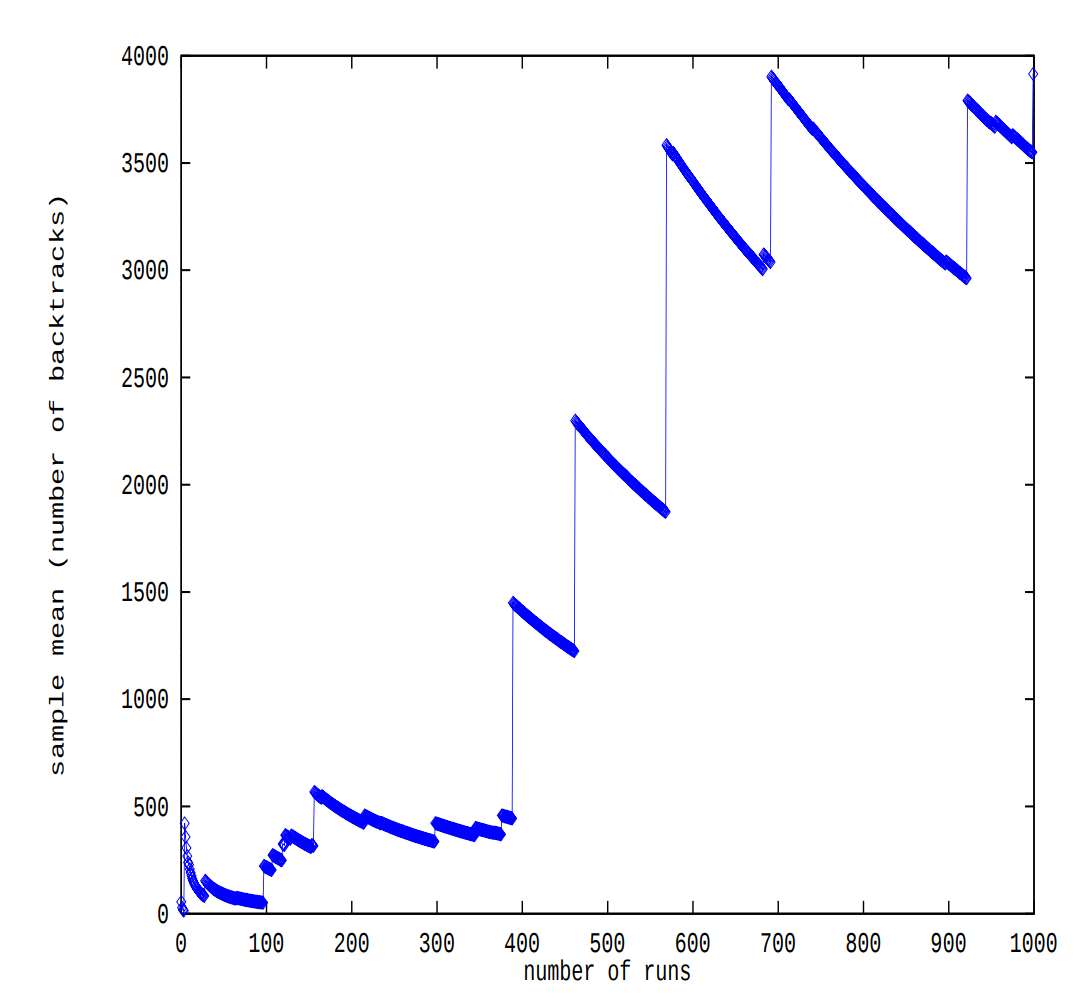
\includegraphics[scale=0.17]{sample_mean_backtracks.png}
    \caption[Sample mean of backtracks]{Sample mean of the number of backtracks required to solve a SAT encoding of the quasigroup completion problem.}
    \label{fig:erratic_mean}
\end{figure}



\subsection{Randomising SAT Solvers}
In order to permit a distribution over backtracks required,
a random element has to be added to the SAT solvers
being analysed. Gomes et al. consider modifications to Satz and Relsat
which are both based on DPLL. These
solvers use a collection of heuristics to determine which
variable to branch on. Gomes et al. define a constant $H$,
such that all variables that are in the top $H$-percent, as evaluated by
the heuristics, are chosen at random with
uniform probability.

\subsection{Pareto-L\'evy Distributions}
\subsubsection{Distributions with infinite moments}
Gomes et al. consider a class of distributions called Pareto-L\'evy distributions which have the following form.
\begin{align*}
    \text{P}(X > x) &\sim Cx^{-\alpha}, \hspace{5pt} x > 0 \footnotemark\\
    C &> 0\\
    0 < &\alpha < 2
\end{align*}
\footnotetext{Here $f(x) \sim g(x)$ is used to mean 
$\lim_{x \to \infty} \frac{f(x)}{g(x)} = 1$}
This means that the distribution decays polynomially in $x$ as opposed to exponentially, as would be the case
for a Gaussian distribution.
An example of a probability distribution with this form is the Cauchy distribution
which is defined as follows.
\begin{equation*}
    \text{Cauchy}(\gamma, \delta) = \frac{1}{\pi}\cdot\frac{\gamma}{\gamma^{2} + (x - \delta)^{2}}
\end{equation*}
For the Cauchy distribution $\alpha = 1$. For the Pareto-L\'evy distribution $\alpha = 0.5$.
\subsubsection{Distribution of Backtracks required by randomised SAT Solvers}
Gomes et al. empirically sample the number of backtracks required to solve a SAT instance for a
few different instances taken from different domains. These domains are the Quasigroup completion problem,
Scheduling, logistics planning and register allocation. For brevity only the scheduling example is shown here
in Figure \ref{fig:scheduling}. This plot shows the probability $\text{P}(X > x)$, where x is the number of backtracks required
to solve the instance on the randomised solver. The scale on the plot is logarithmic so a straight line
implies polynomial decay.
\begin{align*}
    m \cdot \log(x) + b &= \log(\text{P}(X > x))\\
    x^{m} e^{b} &= \text{P}(X > x)\\
    \text{P}(X > x) &\sim Cx^{m}
\end{align*}
Hence we can estimate $\alpha$ from the slope of the line in the plot.

\begin{figure}
    \centering
    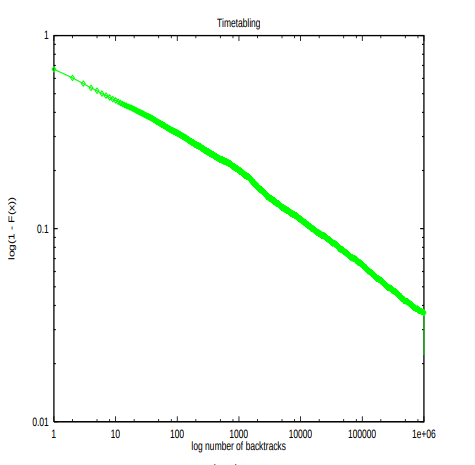
\includegraphics[scale=0.35]{scheduling_tails.png}
    \caption[Distribution of number of backtracks]{Cumulative $\log$ plot of the number of instances solved with a given number of backtracks. Gomes et al. estimates a value of $\alpha = 0.219$ for this problem}
    \label{fig:scheduling}
\end{figure}

\subsection{Motivation for rapid restarts in SAT solvers}
Gomes et al. go on to state that since there is non-negligible probability to the left
side of the distribution then a sequence of many short runs would be more effective than
a single long run. Gomes et al. then empirically validate their claim by modifying Satz and Relsat
to include rapid restarts when a certain number of backtracks is reached.
This results in an order of
magnitude reducing in the time to solve SAT instances,
although the point at which restarting is most
effective depended on the domain of the problem.

\subsection{Points of Caution}
From this we should be cautious to label any given SAT instance as difficult since
the underlying distribution of the number of backtracks required to find a satisfying
assignment has undefined mean and variance. As such we also cannot immediately trust a
sample of runs giving a mean runtime, since the mean does not converge to anything.
Ideally, we should consider the median runtime, which is defined for heavy-tailed distributions
and is therefor more trustworthy in empirical tests.

\section{Phase Transition}
Consider a SAT instance $F$ with few clauses compared to the number of variables,
intuitively this formula has many degrees of freedom and few constraints so
it is highly likely that $F$ will be satisfiable. Furthermore, if we consider
how a run of a backtracking solver would behave on such an instance, since it
only backtracks when it finds a conflict and few conflicts exist then it would
find an assignment without requiring many backtracking steps. If we instead
consider a SAT instance $F'$ with many clauses compared to the number of variables
we can see that a backtracking solver would be spending most of its time applying
unit propagation. Hence in this case also the solver would be able to decide
that $F'$ is not satisfiable quickly.

We call these instances underconstrained and overconstrained respectively.
Work by Cheeseman et al. suggests that all NP-COMPLETE problems have some
order parameter which exhibits a phase transition between underconstrained and 
overconstrained. Furthermore, the hard instances of an NP-COMPLETE problem
occur exactly at the point of the phase transition \cite{cheeseman1991really}.
Here, hardness is measured by the number of backtracking steps that are required
to solve an given instance of an NP-COMPLETE problem. Taking $k$-SAT as an example,
the order parameter is the ratio of the number of clauses to the number of variables
$\frac{m}{n}$ and the hardest instances of $k$-SAT are found at some critical value
$c_k$. This explains how Turner et al. were able to achieve their algorithm,
most random instances are far from the critical value \cite{turner1988almost}.

% ratios for ksat
\subsection{Transition Sharpness}
The phase transition is known to be ``sharp'' \cite{phase_transition}
in the following sense. Let
$U_k(n, m)$ be the uniform distribution over all $k$-CNF formulas with
$n$ variables and $m$ clauses and $c_k$ be the critical value, then
\begin{equation} \label{eq:sharp}
    \mathrm{Pr}_{F \sim U_k(n, m)}[F\text{ is satisfiable}] =
    \begin{cases}
        0 & \frac{m}{n} > c_k \\
        1 & \frac{m}{n} < c_k
    \end{cases}
    \quad\text{as }
    n \to \infty
\end{equation}
For 2-SAT this critical value is known to be $c_2 = 1$, \cite{chvatal1992mick, goerdt1996threshold}.
However, for all $k \geq 3$, no exact value of $c_k$ is known. Although it is known
that $3.003 < c_3 < 4.81$ and $c_3 \approx 4.24$ \cite{crawford1993experimental}
(see Figure \ref{fig:phase_sat_prob}).

\begin{figure}
    \centering
    \hspace{-2cm}
    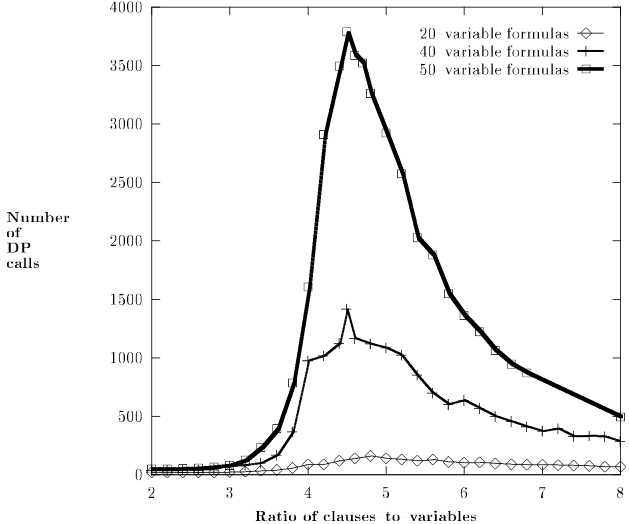
\includegraphics[scale=0.5]{DP_backtracks.png}
    \caption{Median number of backtracks required to solve a 3-SAT instance for varying
    clause ratio \cite{hard_and_easy_distributions}}
    \label{fig:phase_backtracks}
\end{figure}
\begin{figure}
    \centering
    \hspace{-2cm}
    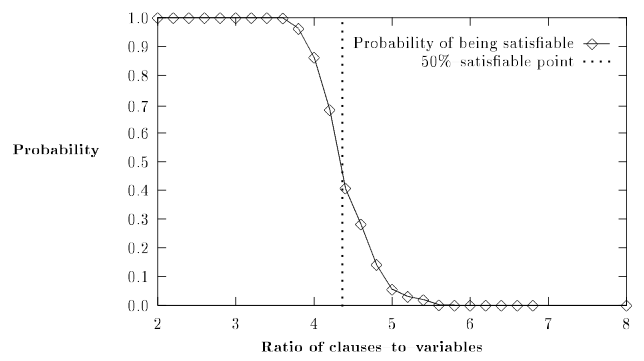
\includegraphics[scale=0.5]{phase_transition_probs.png}
    \caption{Probability that a random 3-SAT instance is satisfiable for varying
    clause ratio \cite{hard_and_easy_distributions}}
    \label{fig:phase_sat_prob}
\end{figure}

For large $n$ only instances close to critical values will be hard
(See Figure \ref{fig:phase_backtracks}).
This fact has been used by Mitchell et al. \cite{hard_and_easy_distributions}
to define probability distributions over $k$-SAT instances that are hard for
the purpose of creating new challenging benchmarks.

\subsubsection{Analogies to Spin Glasses and Statistical Mechanics}
Work by Kirkpatrick uses elements of statistical mechanics and an analogy of
random $k$-SAT to spin glasses to propose a form for phase transition.
Their work suggest that for some fundamental function $f$ and constants $c_k$
and $v$ then
\begin{equation}
    \mathrm{Pr}_{F \sim U_k(n, m)}[F \text{ is satisfiable}] = f\Big(\Big(\frac{m}{n} - c_k\Big) \cdot \frac{n^{1/v}}{c_k}\Big) % check this c_k substitution
\end{equation}
Using empirical methods $f$ and the constants $c_k$ and $v$ can be estimated.
Kirkpatrick et al. estimate $c_3 \approx 4.17$ and $v \approx 1.5$ \cite{kirkpatrick1994statistical}.
We note that this form for the satisfiability probability illustrates that
for any $\frac{m}{n} - c_k \neq 0$ then as $n \to \infty$ the probability tends
to $f(-\infty)$ or $f(\infty)$. If we
have that $\lim_{x \to -\infty}f(x) = 1$ and $\lim_{x \to \infty}f(x) = 0$ then we
can justify Equation \ref{eq:sharp}.


\subsection{Generalisations}
However, most ``in practice'' SAT instances do not have fixed clause length
and instead have many short and long clauses. Work by Gent et al. generalises
the SAT phase transition to mixed-clause instances \cite{phase_transition}.
Consider a probability distribution over the integers $\phi(k)$, let a $\phi$-SAT
formula $F$ be such that for a randomly selected clause $C \in F$
\begin{equation}
    \mathrm{Pr}[|C| = k] = \phi(k)
\end{equation}
i.e. clauses of size $k$ are picked to be in $F$ with probability $\phi(k)$.

Denote the critical value for a particular distribution $c_\phi$. Gent et al.
give a simple upper bound for $c_\phi$. Let $\alpha$ be an assignment chosen
uniformly at random and $C_k$ be an arbitrary clause of length $k$.
For a given distribution of clause lengths $\phi$ we define
$d_\phi$ as follows:
\begin{equation}
    d_\phi = \mathrm{Pr}_{k \sim \phi}[\alpha \text{ satisfies } C_k] = \sum_{k=1}^{\infty}\phi(k) \Big(1 - \Big(\frac{1}{2} \Big)^k \Big)
\end{equation}
If we consider a $\phi$-SAT instance $F = \{C_1, C_2, \dots, C_m\}$
with $m$ clauses then
\begin{align*}
    \mathrm{Pr}[\alpha \text{ satisfies } F] &= \prod_{i = 1}^{m}\mathrm{Pr}[\alpha \text{ satisfies } C_i] \\
    &= d_\phi^m
\end{align*}
Thus, if the number of variables is $n$, then the expected number of satisfying
assignments is $2^n d_\phi^m$. For a formulas to be unsatisfiable as $n \to \infty$
we must have that $2^n d_\phi^m < 1$ or equivalently $2(d_\phi)^{\frac{m}{n}} < 1$.
Rearranging we get $\frac{m}{n} > \frac{-1}{\log_2(d_\phi)}$. Since as $n \to \infty$
all formulas with a clause ratio greater than this are unsatisfiable then we know that
\begin{equation}
    c_\phi \leq \frac{-1}{\log_2(d_\phi)}
\end{equation}
This gives us our desired upper bound.

\section{Backdoors}
\subsection{Formalising Intuitions}
One intuition for why some SAT instances are easy come from the idea
that not all variables are equal. One can consider a dichotomy of variables,
dependent variables and independent variables, where dependent variables are
variables that are needed to encode a specific problem but are simple consequences
of the assignment to the independent variables. As an example, consider a software
verification task, it is likely that there many variables included in the SAT
encoding that are encoding straightforward implications or auxiliary information.
The assignments to these variables can be quickly deduced after the heart
of the combinatorial problem is solved, namely finding an assignment
to the independent variables. As such, 
dependent variables do not contribute to the combinatorial hardness of the instance,
since it is sufficient to find an assignment to the independent variables and the
dependent variables can be determined efficiently from this assignment.\cite{gerevini2003planning}

We can attempt to explain the in practice performance of many SAT solvers
by understanding the effect of having many dependent variables on the complexity
of SAT and by attempting to verify that having many dependent variables is common.
To do this we need a formalism that captures the idea of there being a set
of independent variables and a set of dependent variables that can be derived quickly
from the independent variables.
Work by Williams et al. does exactly this \cite{backdoor_typical}.

A brief mention of notation, for a SAT instance $F$ and a partial assignment $\alpha_S$
to a subset of the variables $S$, let $F[\alpha]$ denote the simplified version of $F$
under the assignment $\alpha_S$.
A backdoor set can then be defined as follows:
\begin{definition}
    A Backdoor set is a subset of variables $S$ such that there
    exists an assignment $\alpha_S$ of the variables in $S$ and $F[\alpha_S]$
    is solvable by a ``sub solver''. \cite{backdoor_typical}
\end{definition}
\begin{definition}
    A sub solver $A$ is an algorithm which has the following properties \cite{backdoor_typical}:
    \begin{itemize}
        \item Given a SAT instances, $A$ either refuses the instance or
        correctly determines that it is satisfiable or unsatisfiable.
        \item $A$ runs in polynomial time.
        \item If for a SAT instance $F$, $A$ does not refuse $F$, then for all
        assignments to the variables $\alpha$, $A$ does not refuse $F[\alpha]$
    \end{itemize}
\end{definition}
An example sub solver could be a solver for 2-SAT \cite{aspvall1979linear},
q-HORN \cite{boros1994recognition} or a modified unit propagation procedure
\cite{davis1960computing}.

We can see that the backdoor set captures our notion of the independent variables
that once assigned allow the dependent variables to be deduced via some sub solver
that is efficient.

\subsection{Complexity for Instances with Small Backdoors}
For a given instance $F$ with $n$ variables, if we knew that
this instance had a backdoor set $S$, we could simply try all the 
partial assignments to $S$, running the sub solver at each step. Since
the sub solver runs in polynomial time, then this would take time 
$\mathcal{O}^{\ast}(2^{|S|})$. So for small $S$ this would be asymptotically faster
than brute force search or backtracking search. Ideally, if we had that
$|S|$ was $\mathcal{O}(\log n)$ then we could solve satisfiability in
polynomial time.

However, this depends on us knowing what the backdoor set $S$ is, which is rarely
the case. Therefore, we need to account for the additional complexity for
finding the backdoor set. Luckily Williams et al. define a deterministic algorithm
that for sufficiently small backdoors finds a backdoor and solves the SAT instance
asymptotically faster than $\mathcal{O}(2^{n})$

The deterministic algorithm can be seen in Algorithm \ref{alg:deterministic}. It
is analogous to iterative deepening search: checking all possible subsets in increasing
order of size and then all assignments to the variables in those subsets. If any
assignment simplifies $F$ to the point where $F[\alpha_S]$ is not refused by $A$ then
we can solve the rest of the instance using $A$. If $A$ finds that $F[\alpha_S]$
is satisfiable, then so is $F$.

\begin{algorithm}
\caption{Deterministic Solver}
\label{alg:deterministic}
\vspace{5pt}
\KwIn{CNF Formula $F$ with $|V| = n$ variables and $m$ clauses, sub solver $A$}
\KwOut{SAT or UNSAT}
\hrulefill\\

\nl \For{$i \in 1,2, \dots, n$}{
    \nl \For{$S \in \{S \subseteq V : |S| = i\}$}{
        \nl \For{$\alpha_S \in \{\text{True}, \text{False}\}^{|S|}$}{
            \nl \If{$F[\alpha_S]$ is not refused by $A$}{
                \nl \If{$A(F[\alpha_S]) = \text{SAT}$}{
                    \nl \Return{} SAT
                }
            }
        }
    }
}
\nl \Return{} UNSAT

\end{algorithm}

To analyse the complexity of Algorithm \ref{alg:deterministic} first let
the size of the smallest backdoor be upper bounded by the function $B(n)$.
We assume that $B(n) \leq \frac{n}{2}$.
Since $A$ runs in $poly(n)$ by definition we can bound the total running time $T(n)$
by the following.
\begin{equation} \label{eq:upper_bound}
    T(n) \leq poly(n)\sum_{i = 1}^{B(n)} \binom{n}{i} 2^i
\end{equation}
Following from our assumption that $B(n) \leq \frac{n}{2}$ then we recognise that
\begin{equation*}
    \sum_{i = 1}^{B(n)} \binom{n}{i} \leq n\cdot\binom{n}{B(n)}
\end{equation*}
and
\begin{equation*}
    \sum_{i = 1}^{B(n)} 2^i \leq 2 \cdot 2^{B(n)}
\end{equation*}
Therefore by combining this with Equation \ref{eq:upper_bound}
we obtain the following upper bound
\begin{align}
    poly(n)\sum_{i = 1}^{B(n)} \binom{n}{i} 2^i &\leq poly(n)\Big(\sum_{i=1}^{B(n)} \binom{n}{i}\Big)\Big(\sum_{i=1}^{B(n)} 2^i \Big) \nonumber\\
    &\leq poly(n) \cdot n \cdot \binom{n}{B(n)} \cdot 2 \cdot 2^{B(n)} \nonumber\\
    &\leq poly(n) \binom{n}{B(n)} 2^{B(n)} \nonumber\\
    &\leq poly(n) \frac{n^{B(n)}}{B(n)^{\frac{B(n)}{2}}} 2^{B(n)} \label{eq:fact_bound}\\
    &\leq poly(n) \Bigg( \frac{2n}{\sqrt{B(n)}} \Bigg)^{B(n)} \label{eq:det_door_bound}
\end{align}

We get arrive at Equation \ref{eq:fact_bound} by realising that
for all $n \in \mathbb{N}$ we have that $B(n)! \geq B(n)^{B(n) / 2}$ and
that $n! / (n - B(n))! \leq n^{B(n)}$

If we consider the case where the size of the smallest backdoor is
logarithmic in $n$ (i.e. $B(n) = \log n$), then Williams et al. derive the
complexity of Algorithm \ref{alg:deterministic} to be the following
\cite{backdoor_typical}:
\begin{equation}
    \Bigg( \frac{n}{\sqrt{\mathcal{O}(\log n)}} \Bigg)^{\mathcal{O}(\log n)}
\end{equation}
Which is asymptotically faster than $\mathcal{O}(2^n)$.

\subsection{Improved Upper Bounds}
However, we note that this can be improved slightly.
In Equation \ref{eq:fact_bound}, Williams et al. use the fact that
$\forall n \in \mathbb{N}: n! \geq n^{n / 2}$. However we state
the following lower bound for the factorial:

\begin{equation} \label{eq:new_fact_bound}
    \forall k \in (1, \infty): \exists \delta \in \mathbb{R}: \forall n \in \mathbb{N}: \delta n! \geq n^{n / k}
\end{equation}
\begin{proof}
    Applying Stirling's approximation of $n!$ we can restate the bound as
    \begin{equation*}
        n^{n / k} \leq \delta\sqrt{2\pi} n^{n + \frac{1}{2}} e^{-n}
    \end{equation*}
    Rearranging we derive the following:
    \begin{equation*}
        n^{n / k - n - \frac{1}{2}} \leq \delta\sqrt{2\pi} e^{-n}
    \end{equation*}
    Taking logs on both sides, we see that
    \begin{equation*}
        (n / k - n - \frac{1}{2})\log n \leq \log (\delta\sqrt{2\pi}) - n
    \end{equation*}
    Rearranging again
    \begin{equation} \label{eq:constant_lhs}
        \Big(\frac{1}{k} - 1\Big)n \log n + n - \frac{1}{2}\log n \leq \log (\delta\sqrt{2\pi})
    \end{equation}
    It is clear that if $k > 1$ then $(\frac{1}{k} - 1) < 0$, which means
    that the $n\log n$ term dominates as $n \to \infty$. Hence the LHS of Equation
    \ref{eq:constant_lhs} has a finite maximum.
    To complete the proof we simply choose $\delta$ to be
    \begin{equation}
        \delta = \max_{n \in \mathbb{N}} \Bigg\{
        \frac{1}{\sqrt{2\pi}}\exp \Big\{ \Big(\frac{1}{k} - 1 \Big)n \log n + n - \frac{1}{2}\log n \Big\} \Bigg\}
    \end{equation}
\end{proof}

We can then use the Inequality \ref{eq:new_fact_bound} and \ref{eq:fact_bound}
to derive a new upper bound on the running time of Algorithm \ref{alg:deterministic} for all $k > 1$.
\begin{equation} \label{eq:new_det_bound}
    T(n) \leq poly(n)\Big( \frac{2\delta n}{B(n)^{1 / k}} \Big)^{B(n)}
\end{equation}
So if we again consider the case where $B(n) = \mathcal{O}(\log n)$, then
for all $k > 1$ the time complexity is
\begin{equation}
   \Bigg( \frac{n}{\mathcal{O}(\log n)^{1 / k}} \Bigg)^{\mathcal{O}(\log n)}
\end{equation}
Which, for $1 < k < 2$ is an improvement over the bound achieved by
Williams et al.

\subsection{Empirical Results}
Williams et al. also state that for $B(n) = \frac{n}{4.404}$
Algorithm \ref{alg:deterministic} runs in time $\mathcal{O}(c^n)$ for
some $c < 2$. Hence, SETH implies that there must exist some infinite
set of SAT instances where the backdoor size is larger than $\frac{n}{4.404}$.
Granted, this tells us nothing about the proportion of SAT instances that do
have small backdoor sets, although we should perhaps question whether
it is reasonable to expect to find small backdoors reliably.

However, Williams et al. use a modified version of
Satz-rand \cite{kautz1999unifying} to effectively implement
Algorithm \ref{alg:deterministic} and experimentally verify the existence of small backdoors
for a few benchmark instances. The results of applying this to a few
SAT benchmarks can be seen in Table \ref{tab:backdoor_sizes}.
We can see that these practical instances have backdoor sets that are
much smaller than their total number of variables. This provides support
to the idea that the performance of modern SAT solvers comes in part
from their ability to exploit small backdoor sets in practical instances.

However, it is not clear from Table \ref{tab:backdoor_sizes} that we can expect
to find small backdoors in all SAT instances. In particular if we consider the
instances with the smallest fractional backdoor set sizes we see that they either have
largest clause ratios or smallest clause ratios. This means that, although we do not know the exact
phase transition for these instances, they likely lie far from the phase transition and therefore
we already expect them to be easier (see Figure \ref{fig:phase_backtracks}).

More work is needed to examine if there are small backdoor sets at the point of the
phase transition and to examine potential links between the distance from the phase
transition and sizes of the smallest backdoor sets.

\begin{table}[]
    \centering
    \begin{tabular}{l c c c c c}
        \toprule
        instance name & \#vars & \#clauses & backdoor size & fraction & clause ratio\\
        \midrule
        logistics.d & 6783 & 437431 & 12 & 0.0018 & 64.5\\
        3bitadd\_32 & 8704 & 32316 & 53 & 0.0061 & 3.71\\ 
        pipe\_01 & 7736 & 26087 & 23 & 0.0030 & 3.37\\
        qg\_30\_1 & 1235 & 8523 & 14 & 0.0113 & 6.90\\
        qg\_35\_1 & 1597 & 10658 & 15 & 0.0094 & 6.67\\
        \bottomrule
    \end{tabular}
    \caption{Sizes of Backdoors in SAT benchmark instances \cite{backdoor_typical}}
    \label{tab:backdoor_sizes}
\end{table}

\subsection{Parameterization by Backdoor Size}
Another approach to attempting to quantify the effect of backdoors is to
consider the complexity of SAT, parameterized by the size of the backdoor.
This can potentially be a little confusing since we already usually express
the complexity in terms of the parameter $n$ and will now be introducing
a different parameter $k$.

\nomenclature[z-FPT]{FPT}{Fixted Parameter Tractable}

% introduce fpt
Ideally what we want is an algorithm that is in FPT, so
if $k$ is the size of the backdoor and $x$ is the SAT instance then the
algorithm runs in $\mathcal{O}(f(k)|x|^{c})$ for some constant $c \in \mathbb{R}^{+}$
that does not depend on $k$ and some computable function $f$.
If we consider the complexity of Algorithm \ref{alg:deterministic} and its
complexity in Inequality \ref{eq:new_det_bound}, if we try to reformulate
this complexity into the FPT form we will see that we are unable to get the
constant $c$ to be independent of $k$ (which is referred to as $B(n)$ in Inequality \ref{eq:new_det_bound}).

% detecting backdoors is w2 hard
Work by Nishimura et al. \cite{nishimura2004detecting} and Gaspers et al.
\cite{gaspers2016backdoors} show that detecting backdoors is $W[2]$-HARD
for a range of popular sub solvers. Therefore, since Algorithm
\ref{alg:deterministic} is general for all sub solvers it is also at least
$W[2]$-HARD. So unless FPT$ = W[2]$ then we should not expect
to find FPT algorithms for backdoor sets.

% fpt for strong and deletin
However, Nishimura et al. also show that with sub solvers
for 2-SAT and Horn formulas, strong backdoor sets can be found in FPT time
and that with sub solvers for q-horn \cite{boros1994recognition} finding strong
backdoor sets is $W[2]$-HARD
\cite{nishimura2004detecting}. However, work by Ramanujan et al. show
that for a q-Horn sub solver deletion backdoors
can also be found in FPT time \cite{ramanujan2017linear}.

\begin{definition}
    A strong backdoor, for a sub solver $A$ and
    a SAT instance $F$ with a variable set $V$, is
    a subset $S \subseteq V$ such that for all assignments $\alpha_S$ to
    the variables in $S$ $F[\alpha_S]$ is not refused by the sub solver $A$.
\end{definition}

\begin{definition}
    A deletion backdoor, for a sub solver $A$ and a SAT instance $F$
    with a variable set $V$, is a subset $S \subseteq V$ such that
    $F_S = \bigcup_{C \in F}\{\{l \in C : vars(l) \notin S \}\}$
    is not refused by $A$.
\end{definition}

An important observation is that for the same sub solver $A$, every
deletion backdoor is also a strong backdoor. This follows from the fact
that for any assignment to a variable $v \in S$, either all clauses including
a positive literal of $v$ are removed and all instances of $\neg v$ are removed
or all clauses including $\neg v$ are remove and all instances of the positive
literal $v$ are removed. So for either assignment to $v$ all positive and
negative occurrences of $v$ are removed from $F$. So therefore for any
assignment $\alpha_S$ to a deletion backdoor $S$, $F[\alpha_S] \subseteq F_S$.
So any sub solver not refusing $F_S$ must also not refuse $F[\alpha_S]$ for
all $\alpha_S$. Hence, any algorithm that detects strong backdoors can
also be easily modified to detect deletion backdoors.

However, a drawback of deletion backdoors is that the smallest deletion
backdoor can be arbitrarily larger than the smallest strong backdoor.
The following example from Gaspers et al. illustrates this.
\begin{equation}
    F = \bigcup_{i = 1}^{n} \{\{x_{i,1}, x_{i,2}, x_{i,3}, a\},
    \{\neg x_{i,1}, \neg x_{i,2}, \neg x_{i,3}, \neg a\}\}
\end{equation}
If we consider the sub solver $A$ to the application of the
pure literal rule from DP \cite{davis1960computing}, then we can see
that $\{a\}$ is a strong backdoor, but there is no deletion backdoor set
smaller than $n$.

If we find a deletion backdoor set of size $k$, we can
solve the SAT instance in time $\mathcal{O}(2^{k}|x|^{c})$ by checking
all assignments to the deletion backdoor. What remains is to find
a deletion backdoor in FPT time.
A summary of of the results by
Nishimure et al., Ramanujan et al. and Gaspers et al. can be seen in Table \ref{tab:backdoor_fpt}. We see that as the ``power'' of the sub solver increases,
the difficulty of finding a backdoor increases.

\begin{table}[]
    \centering
    \begin{tabular}{l c c c}
        \toprule
        Sub solver & weak backdoor & strong backdoor & deletion backdoor \\
        \midrule
        Horn & $W[2]$-HARD & FPT $\mathcal{O}(2^k |x|)$ & FPT $\mathcal{O}(2^k |x|)$\\
        2-CNF & $W[2]$-HARD & FPT $\mathcal{O}(3^k |x|)$ & FPT $\mathcal{O}(3^k |x|)$\\
        q-Horn & $W[2]$-HARD & $W[2]$-HARD & FPT $\mathcal{O}(12^k k^5 |x|)$ \\
        \bottomrule
    \end{tabular}
    \caption{Summary of FPT results for different backdoors and sub solvers 
    \cite{nishimura2004detecting, ramanujan2017linear, gaspers2016backdoors}}
    \label{tab:backdoor_fpt}
\end{table}

\section{Conclusions and Further Work}

% recap solvers
In Chapter \ref{chap:solvers} we covered a few of the most prominent algorithms
and their corresponding solvers. However, in the worst case these solvers
could take exponential time in the number of variables in the input.
This gives the impression that SAT is infeasible to solve in practice
and results covered in Chapter \ref{chap:complexity} show that the exact worst case
complexity of SAT is related to the exact complexity of other NP-COMPLETE problems
and also related to the exact complexity of some problems in P.
This leads us to believe that improving the worst case complexity of SAT is a challenging problem, albeit,
perhaps less challenging than showing that the complexity cannot be improved.

However, in this Chapter we see that the worst case behaviour can be confined
to a specific region of the input space, namely where the clause ratio is close to phase transition.
Due to the sharpness of the phase transition, large SAT instances that are not close to the phase
transition will with high probability either be satisfiable or unsatisfiable, depending on the side
of the phase transition that the instance is on.

Furthermore, we see that the complexity can be improved if we can guarantee the existence
of small backdoor sets and finding certain types of backdoor sets is fixed parameter tractable.
Additionally, empirical studies find that small backdoor sets are often prevalent in
industrial SAT instances, providing another explanation for why they can be solved
quickly. It is not known whether the prevalence of small backdoor sets and the distance
from the phase transition point are related and this could be explored in further work.

Therefore, taking these two aspects into account it becomes clearer why many industrial SAT instances can
be solved significantly faster than their worst case complexities would suggest.
Since all NP-COMPLETE problems can be reduced to SAT, this also suggests that many
other NP-COMPLETE problems exhibit the same behaviour.
Thus, one practical technique for dealing with NP-COMPLETE problems in practice
would be to reduce the problem to SAT and then use a SAT solver similar to one discussed
in Chapter \ref{chap:solvers}.
